\documentclass[12pt, a4paper]{article}
\usepackage[utf8]{inputenc}
\usepackage[russian]{babel}
\usepackage[pdftex]{graphicx, color}
\usepackage{amsmath, amsfonts, amssymb, amsthm}
\usepackage[left=2cm,right=2cm,top=1.5cm,bottom=2cm]{geometry}
\usepackage{indentfirst}

\usepackage{setspace}
\onehalfspacing
\graphicspath{{pics/}}

\begin{document}
    \begin{singlespace}
    \begin{center}
        
\includegraphics[height=3cm]{msu.png}

        {\large\textbf{Отчёт по лабораторной работе по курсу ММАТ\\
        <<Векторные представления слов, тематическое моделирование. Анализ тональности.>>}}

        \vspace{0.3cm}

        \textit{\textbf{Аят Оспанов}}

        517 гр., ММП, ВМК МГУ, Москва

        8 мая 2017 г.
    \end{center}
    \end{singlespace}

    \tableofcontents

    \section{Постановка задачи}
        \subsection{Классификация текстовой коллекции EUR-lex}
            Дана коллекция документов EUR-lex. Датасет EUR-lex предлагается в виде двух файлов, \verb|eurlex_data.txt| и \verb|eurlex_labels.txt|. Файл с данными содержит два столбца, первый -- идентификатор документа, второй -- сам документ. Файл с метками состоит из трёх столбцов, первый -- имя метки класса, второй -- документ, к которому эта метка относится (у каждого документа может быть несколько меток классов), третий -- константа 1, которую можно игнорировать.

            Для каждого документа из датасета нужно определить классы, к которым этот документ будет относится. Для этого надо сделать следующие шаги:
            \begin{itemize}
                \item Предобработка данных
                \item Создание признакового пространства, описывающее датасет
                \item Классифицировать датасет с помощью алгоритмов классификаций
                \item Посчитать метрики качества ROC AUC и PR AUC
            \end{itemize}

        \subsection{Визуализация признакового пространста}
            В этом пункте нужно визуализировать векторы, полученные с помощью word2vec, и матрицу <<слова-темы>>, полученную с помощью тематического моделирования. Требуется, чтобы визуализация была наглядной, давала какую-то информацию о данных и была, по возможности, красивой.

        \subsection{Анализ тональности текстов постов Twitter}
            Дан датасет постов из Twitter. Датасет содержит слудющие столбцы:
            \begin{itemize}
                \item ItemID -- id документа
                \item Sentiment -- класс (0 или 1)
                \item SentimentSource -- ресурс, откуда был взят датасет
                \item SentimentText -- текст документа.
            \end{itemize}

    \section{Классификация текстовой коллекции EUR-lex}
        \subsection{Предобработка данных}
            Данные из EUR-lex содержат уже обработанные данные представленные в виде токенов. Поэтому особой обработки над текстами не проводилось. Была сделана лишь следующая обработка:
            \begin{itemize}
                \item Были удалены стоп-слова. Стоп-слова были взяты из библиотеки \verb|nltk|\\
                (\verb|nltk.stem.snowball.stopwords|). Были взяты все языки, которые были в библиотеке, т.к. язык документов не один и определению нами не подлежит.

                \begin{singlespace}
                    \begin{center}
                        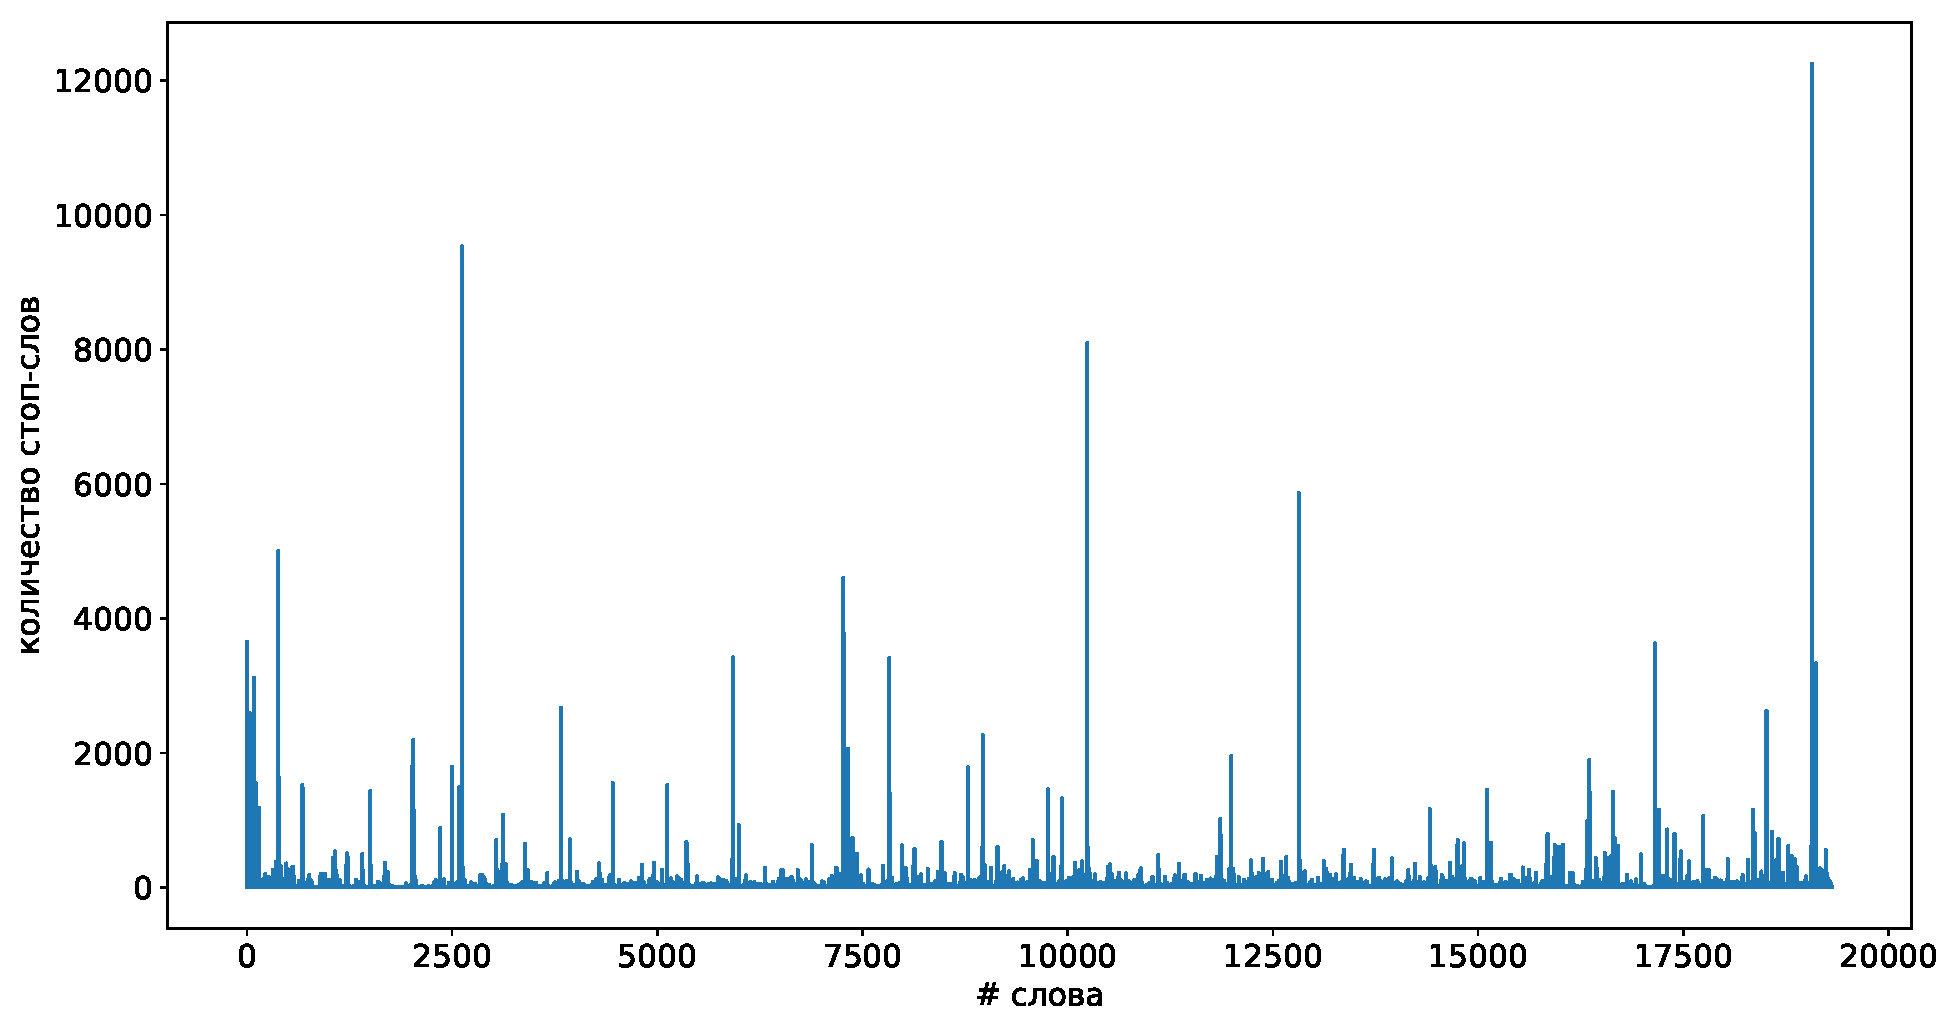
\includegraphics[width=17cm]{diff.pdf}

                        \textit{График количества стоп-слов для каждого документа}
                    \end{center}

                    \begin{center}
                        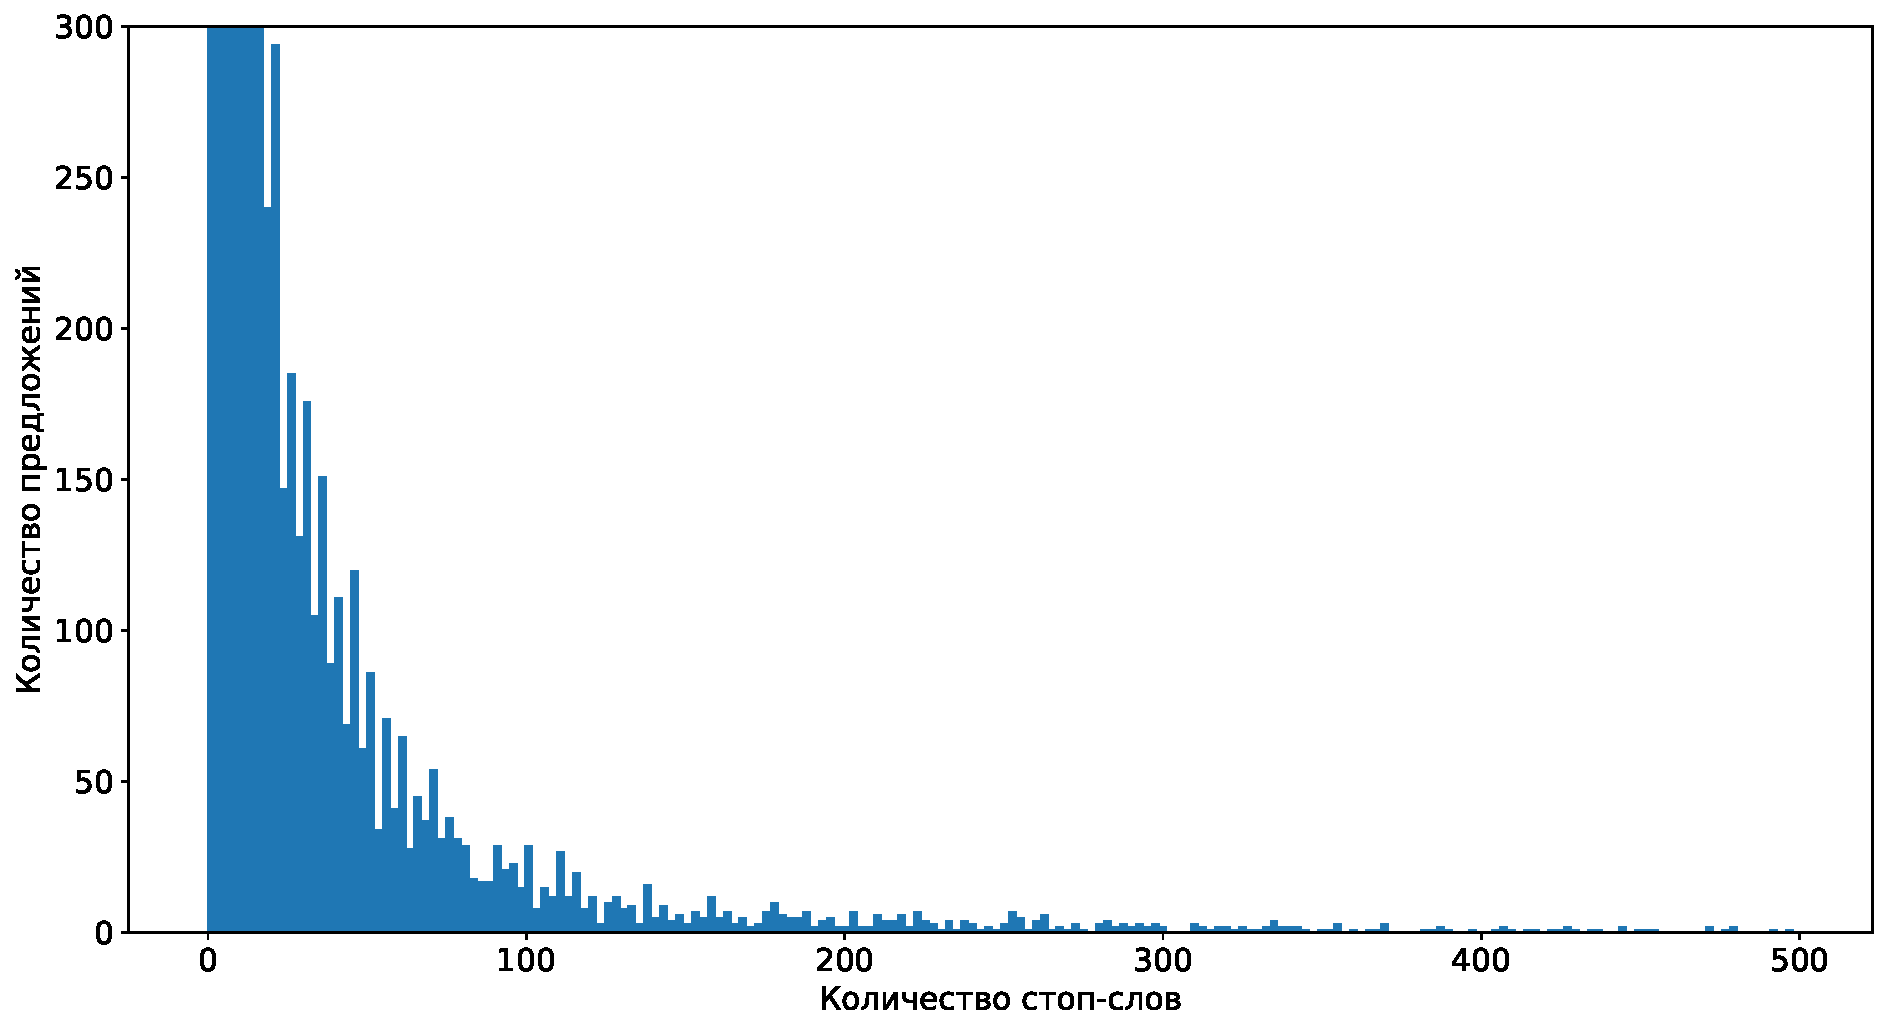
\includegraphics[width=17cm]{diff_dist.pdf}

                        \textit{График плотности документов в зависимости от количества стоп-слов (ордината была ограничена 300 словами)}
                    \end{center}
                \end{singlespace}

                Из графиков видно, что изначальный датасет тексты обработаны, но не удалены стоп-слова.

                \item Токены были отстемлены. Стемминг изпользовался только английский, т.к. стемминг очень долго выполняется. Стеммер брался Snowball из \verb|nltk|\\ (\verb|nltk.stem.snowball.EnglishStemmer|)
            \end{itemize}

            Лемматизация не использовалась по двум причинам: первая -- очень долго работает, вторая -- существует только для английского языка.

        \subsection{Создание признакового пространства}
            Были созданы четыре признаковых пространства:
            \begin{itemize}
                \item Word2Vec

                Для создания пространства, полученного с помощью Word2Vec была использована библиотека \verb|gensim|. А именно модель \verb|models.Word2Vec| с размером вектора 300. Word2Vec возвращает вектор для слова, поэтому бралось среднее по всем словам из документа. Таким образом пространство для документа -- среднее по всем векторам слова документа, полученных с помощью Word2Vec

                \item Тематическое моделирование

                Для создания пространства, полученного с помощью тематического моделирования была использована библиотека \verb|gensim|. А именно модель \verb| models.LdaModel| с 300 темами. В итоге модель возвращает вероятность принадлежности предложения к каждой теме. Пространство для документа -- вероятности принадлежности документа к каждой теме.

                \item Doc2Vec

                Для создания пространства, полученного с помощью Doc2Vec была использована библиотека \verb|gensim|. А именно модель \verb|models.Doc2Vec| с размером вектора 300. Пространство генерировалось аналогично Word2Vec.

                \item Tf-idf + SVD

                Для создания пространства, полученного с помощью Tf-idf была использована библиотека \verb|sklearn|. А именно модель \verb| feature_extraction.text.TfidfVectorizer|. Далее матрица tf-idf сжималось с помощью \verb|TruncatedSVD| из \verb|sklearn.decomposition| до размера 300. В итоге получаем пространство из сжатого до 300 признаков tf-idf.

            \end{itemize}

        \subsection{Классификация}
            Для классификации использовалась логистическая регрессия. Логистическая регрессия использовалась из \verb|sklearn|. Но так как логистическая регрессия -- бинарный классификатор, использовался обертка-классификатор OneVsRest также из \verb|sklearn|. Классификатор использовался с параметрами по-умолчанию.

            В итоге получились следующие результаты:

            \begin{center}
            \begin{tabular}{| l | c | c |}
                \hline
                \textbf{Признаковое пространство} & \textbf{ROC AUC} & \textbf{PR AUC} \\
                \hline
                \textbf{Word2Vec} & 0.97129 & 0.52899 \\
                \textbf{Тематическое моделирование} & 0.92817 & 0.26927 \\
                \textbf{Doc2Vec} & 0.97101 & 0.51168 \\
                \textbf{Tf-idf + SVD} & 0.95058 & 0.44940 \\
                \hline
            \end{tabular}
            \end{center}

            Из таблицы видно, что PR AUC гораздо меньше, чем ROC AUC. Это связано с тем, что Precision-Recall чувствителен к распределению классов. У нас многоклассовая классификация и классы распределены не равномерно и таким образом мы получаем такой маленький PR AUC.

        \subsection{Сравнение предсказаний}
            Был реализован метод, который показывает предсказанные метки для документа. Пример данного метода показан в таблице:
            \begin{center}
            \begin{tabular}{| l | l |}
                \hline
                \textbf{Метод} & \textbf{Классы}\\
                \hline
                \textbf{Метки объекта} & \texttt{ec\_agreement, environmental\_cooperation, environmental\_protection,}\\
                &\texttt{pollution\_control\_measures, rhine\_valley}\\
                \hline
                \textbf{Word2Vec} & \texttt{ec\_cooperation\_agreement, united\_states, economic\_cooperation,}\\
                &\texttt{ec\_agreement, cooperation\_agreement }\\
                \hline
                \textbf{Тематическое} & \texttt{ec\_agreement, protocol\_to\_an\_agreement, ec\_cooperation\_agreement,} \\
                \textbf{моделирование} & \texttt{ec\_association\_agreement, trade\_agreement }\\
                \hline
                \textbf{Doc2Vec} & \texttt{ec\_cooperation\_agreement, economic\_cooperation,} \\
                &\texttt{united\_states, eu\_country, cooperation\_agreement }\\
                \hline
                \textbf{Tf-idf + SVD} & \texttt{ec\_cooperation\_agreement, ec\_agreement, eu\_country,} \\
                &\texttt{economic\_cooperation, cooperation\_policy }\\
                \hline
            \end{tabular}
            \end{center}

    \section{Визуализация признакового пространста}
        \subsection{Word2Vec}
            \begin{singlespace}
                \begin{center}
                    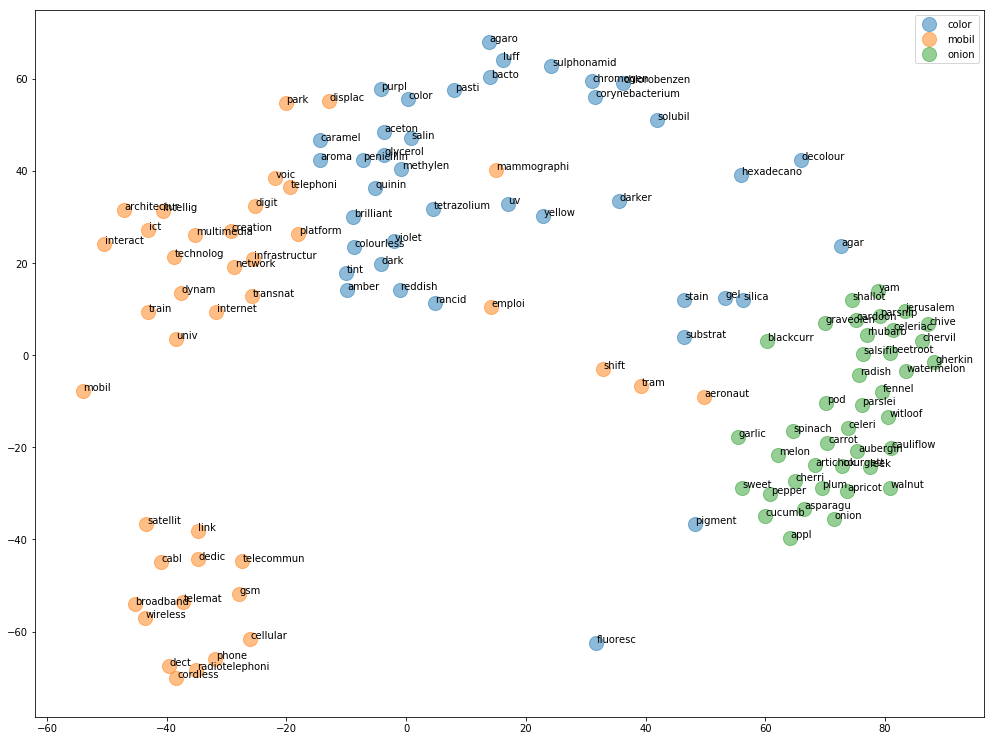
\includegraphics[width=17cm]{w2v.png}

                    \textit{Визуализация для Word2Vec}
                \end{center}
            \end{singlespace}

            Для визуализации векторов, полученных с помощью Word2Vec были выбраны 3 слова, значения которых далеки друг от друга: \textit{color, mobil, onion}. Далее брались по 45 близких слов к каждому слову. Для каждого их всех слов считался вектор с помощью Word2Vec размера 100. Затем просторанство этих векторов были уменьшены до пространства размерности 2 с помощью t-SNE преобразования.

            В итоге получились связные кластера (т.к. мы брали бликие слова) и эти кластера лежат по отдельности друг от друга (т.к. мы брали 3 слова (элементы каждого кластера) далеких друг от друга). Также, если посмотреть на сами слова, то видно, что они похожи или близки по значению. Таким образом можно сказать, что Word2Vec преобразует слова в вектора таким образом, что он ``учитывает'' их значения

        \subsection{LDA}
            \begin{singlespace}
                \begin{center}
                    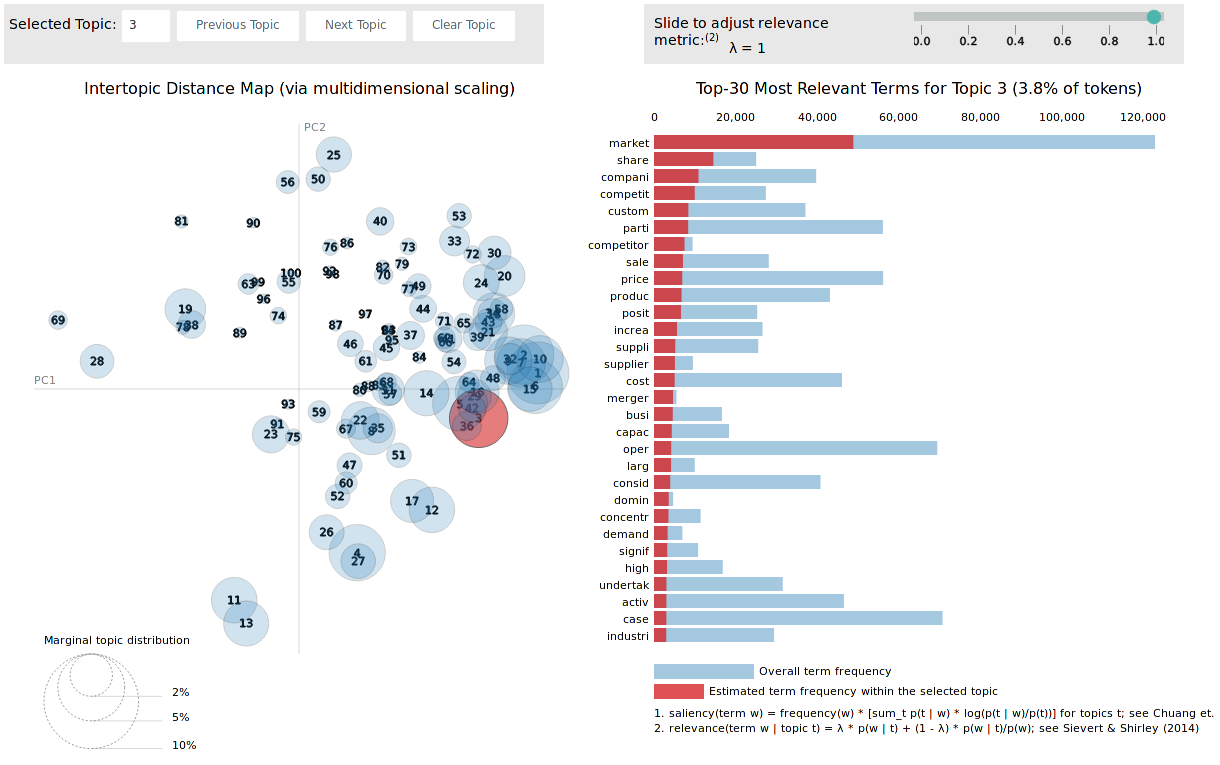
\includegraphics[width=17cm]{lda.png}

                    \textit{Визуализация LDA}
                \end{center}
            \end{singlespace}

            Визуализация тематической модели LDA была сделана с помощью библиотеки \verb|pyLDAvis|. Модель LDA обучалась для 100 тематик, чтобы визуализация была понятной и незагроможденной.

            На левом графике визуализации изображено взаимное расположение тематик в проекции на двумерное пространство. При наведении на тематику отрисовывается правый график. На правом графике изображена гистограмма распределний Топ-30 релевантных слов тематики. Красным цветом изображены количества слов в данной тематике, синим -- количество данных слов в корпусе.

    \section{Анализ тональности текстов постов Twitter}
        \subsection{Предобработка данных}
            Из датасета постов из Twitter нам нужны всего два столбца: Sentiment -- класс (0 или 1) и SentimentText -- текст документа.

            Над данными (SentimentText) была проведена следующая обработка:
            \begin{itemize}
                \item Были оставлены только буквы и цифры. Остальные символы были удалены. Использовалось регулярное выражение ``\verb|\W|''
                \item Были удалены стоп-слова. Стоп-слова использовались встроенные в TfidfVectorizer из \verb|sklearn|
                \item Токены были отстемлены. Стемминг изпользовался английский. Стеммер брался PorterStemmer из \verb|gensim| (\verb|parsing.porter.PorterStemmer|)
            \end{itemize}

            Лемматизация не использовалась по очень простой причине: в Twitter люди пишут не всегда грамматически верно и много сленга.

        \subsection{Создание признакового пространства}
            Были созданы два пространства:
            \begin{itemize}
                \item Tf-idf

                Для создания пространства, полученного с помощью Tf-idf была использована библиотека \verb|sklearn|. А именно модель \verb| feature_extraction.text.TfidfVectorizer|. Матрица не сжималась и использовалась полностью.

                \item Word count

                Для создания пространства, полученного с помощью word count была использована библиотека \verb|sklearn|. А именно модель \verb| feature_extraction.text.CountVectorizer|. Матрица не сжималась и использовалась полностью.

            \end{itemize}

        \subsection{Классификация}
            Для классификации использовались логистическая регрессия (\verb|LogisticRegression|) и наивный байес (\verb|MultinomialNB|). Классификаторы использовались из \verb|sklearn|. Классификаторы использовались с параметрами по-умлочанию.

            Наивный байес проверялся на двух признаковых пространствах. Хотя в документации и написано, что для MultinomialNB предпочтительнее целочисленное пространство и он работает на них хорошо, но может работать и на tf-idf, tf-idf показал результаты чуть лучше.

            Также я предположил, что если оставлять все символы, то качество классификации улучшится. Предположение подтвердилось, но увеличение точности оказалось всего лишь 0.1\%.

            В итоге получились следующие результаты:

            \begin{center}
            \begin{tabular}{| l | l | c | c |}
                \hline
                \textbf{Классификатор} & \textbf{Признаковое пространство} & \textbf{ROC AUC} & \textbf{PR AUC} \\
                \hline
                \textbf{Логистическая регрессия} & \textbf{tf-idf} & 0.86034 & 0.85464 \\
                \textbf{Логистическая регрессия} & \textbf{tf-idf без фильтрации} & 0.86165 & 0.85791 \\
                \textbf{Наивный байес} & \textbf{word count} & 0.84231 & 0.83520 \\
                \textbf{Наивный байес} & \textbf{tf-idf} & 0.84359 & 0.83932 \\
                \textbf{Наивный байес} & \textbf{tf-idf без фильтрации} & 0.84811 & 0.84520 \\
                \hline
            \end{tabular}
            \end{center}

            На таблицы видно, что в случае двуклассовой классификации PR AUC примерно равняется ROC AUC. Это объясняется тем, что у нас классы одинаково распределены.

        \subsection{Визуализация}
            Для интереса попробуем нарисовать облако позитивных и негативных слов.
            \begin{singlespace}
                \begin{center}
                    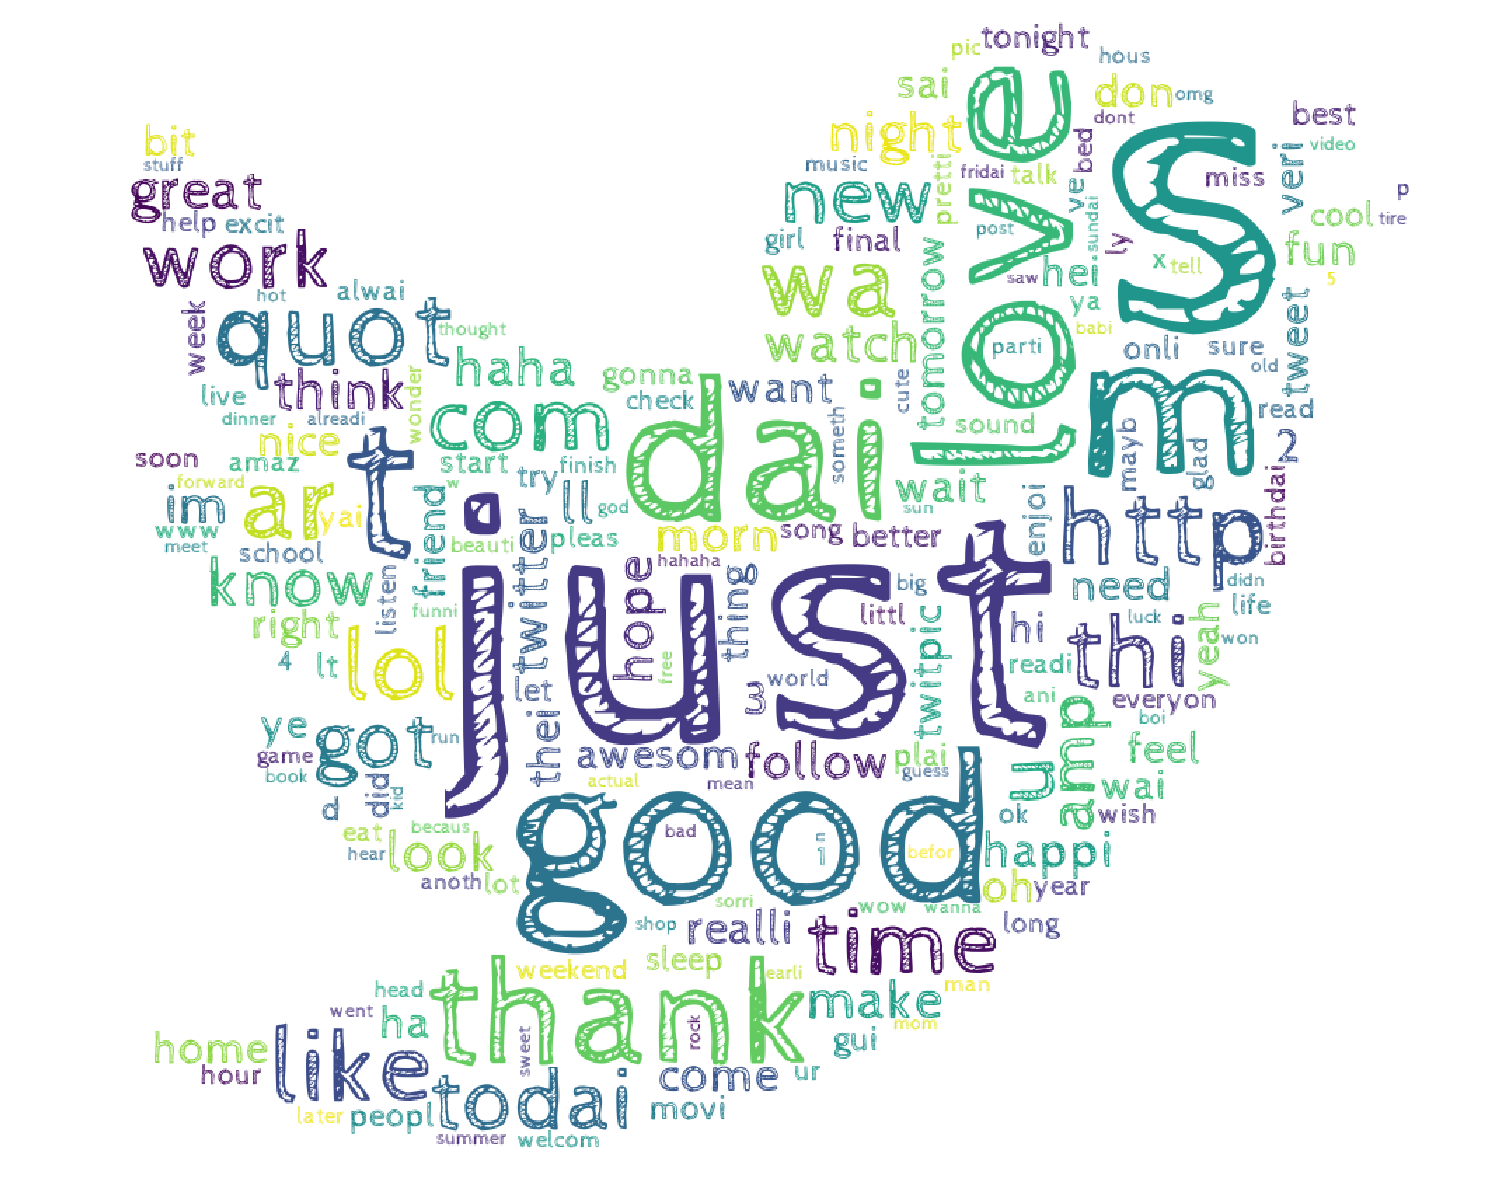
\includegraphics[height=11cm]{twitter_wordcloud_pos.png}

                    \textit{Облако позитивных слов}

                    \vfill

                    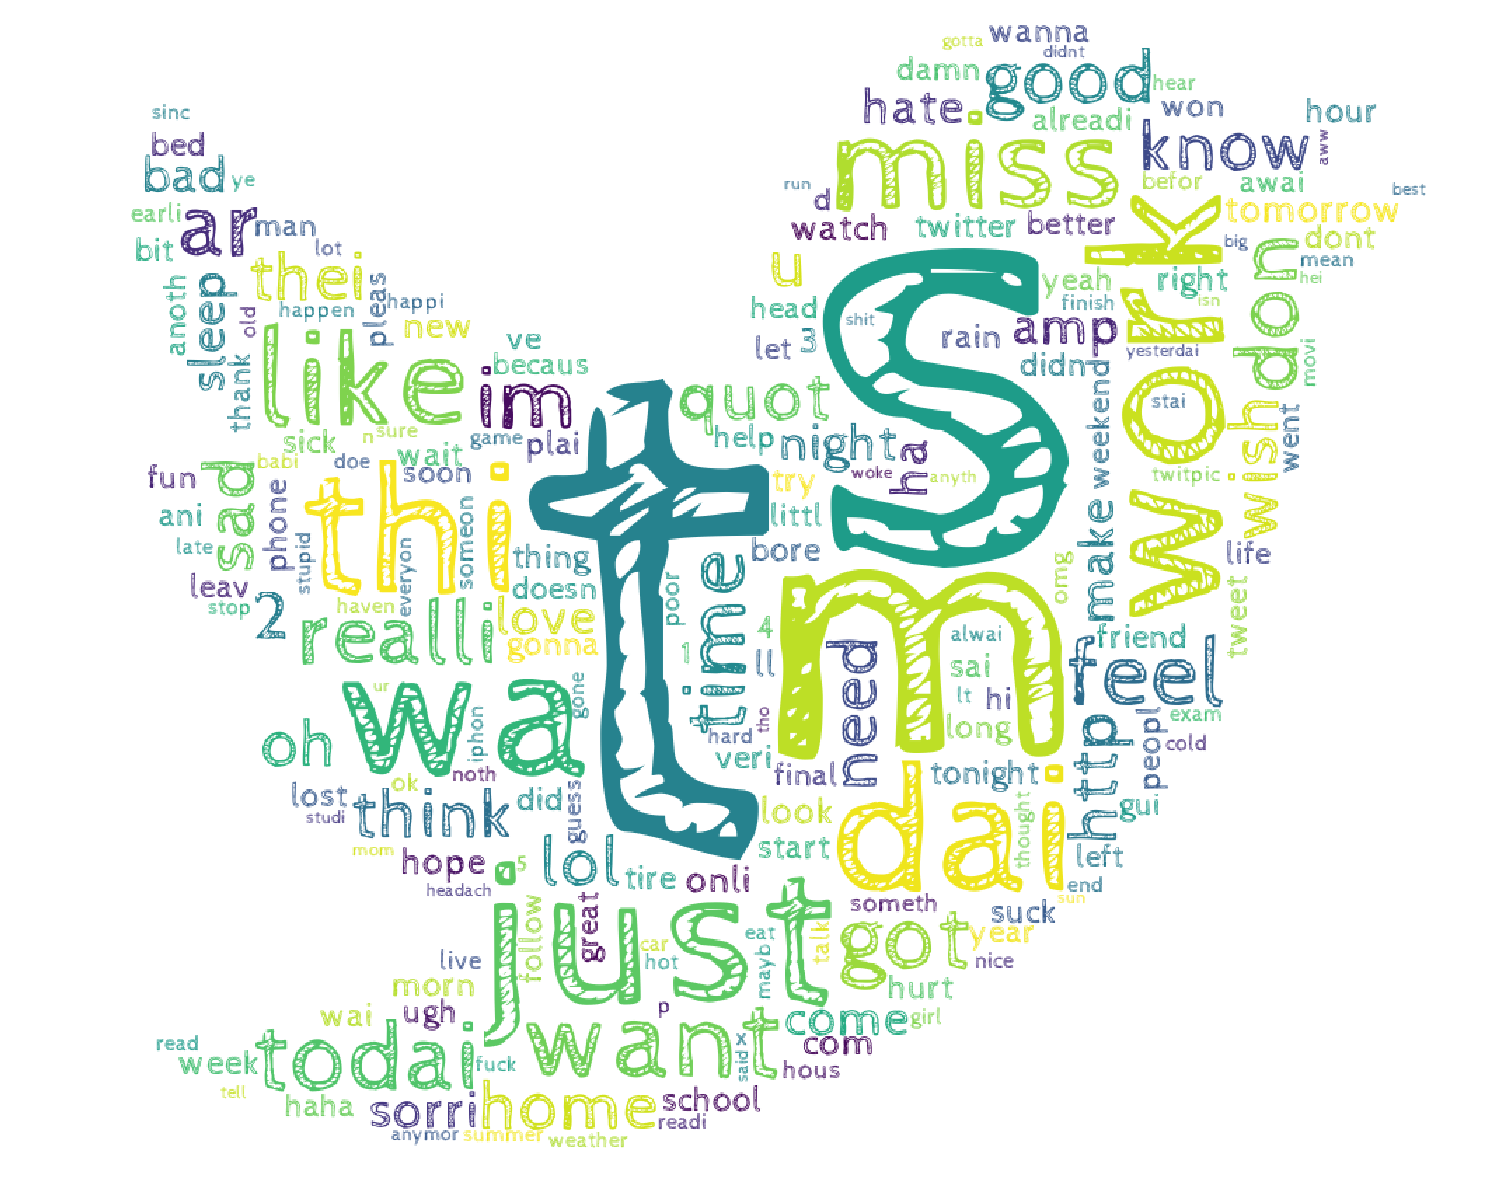
\includegraphics[height=11cm]{twitter_wordcloud_neg.png}

                    \textit{Облако негативных слов}
                \end{center}
            \end{singlespace}

    \section{Заключение}
        В данной работе с помощью методов, изученных в курсе были сделаны задачи классификации текстов и определения тональности текстов. Также:
        \begin{itemize}
            \item были опробованы методы получения векторного представления слов: Word2Vec и Doc2Vec
            \item был опробован метод LDA тематического моделирования
            \item были визуализированы результаты работ методов Word2Vec и LDA
            \item были использованы библиотеки для работы с текстами nltk и gensim
            \item были использованы разные методы классификации и обработки текстов
        \end{itemize}

\end{document}
